% !TeX program = xelatex
\documentclass[12pt,twoside,openany]{book}
\setlength{\parskip}{6pt}

% ==================================================
% ================== FONT ==========================
% ==================================================
\usepackage{fontspec}
\setmainfont{Times New Roman}
% ==================================================
% ================== KHỔ GIẤY 19x27 =================
% ==================================================
\usepackage{geometry}
\geometry{
	paperwidth=19cm,
	paperheight=27cm,
	top=2cm,
	bottom=2cm,
	inner=3cm,
	outer=2cm,
	headsep=1.27cm,
	footskip=1.27cm,
	twoside
}

% ==================================================
% ============== CĂN ĐOẠN & GIÃN DÒNG =============
% ==================================================
\usepackage{enumitem}
\usepackage{ragged2e}
\justifying
\setlength{\parindent}{0.6cm}
\setlength{\parskip}{6pt}
\linespread{1.0}
\raggedbottom

% ==================================================
% ============== CÂU HỎI ÔN TẬP =============
% ==================================================
\usepackage{titlesec}

\titleformat{\section}[block]
{\normalfont\bfseries\fontsize{12}{14}\selectfont\centering}
{}
{0pt}
{}

\titlespacing*{\section}
{0pt}
{16pt}
{16pt}

% ==================================================
% ================== HÌNH ẢNH & BẢNG ===============
% ==================================================
\usepackage{graphicx}
\usepackage{float}
\usepackage[most]{tcolorbox}
\usepackage{caption}
\usepackage{subcaption}
\usepackage{booktabs}
\usepackage{array}
\usepackage{tabularx}
\usepackage{enumitem}
\usepackage{amsmath}
\numberwithin{equation}{chapter}

\renewcommand{\figurename}{Hình}
\renewcommand{\tablename}{Bảng}

% ---- Caption size 11 ----
\DeclareCaptionFont{capfont}{\fontsize{11}{13}\selectfont}

\captionsetup[figure]{
	font=capfont,
	labelfont=bf,
	labelsep=period,
	justification=centering
}

\DeclareCaptionLabelFormat{tablebold}{\textbf{#1~#2}}
\captionsetup[table]{
	font=capfont,
	labelformat=tablebold,
	labelsep=period,
	justification=centering
}

% ---- Nội dung bảng size 11 ----
\setlength{\extrarowheight}{3pt}
\AtBeginEnvironment{tabular}{\fontsize{11}{13}\selectfont}
\AtBeginEnvironment{tabularx}{\fontsize{11}{13}\selectfont}

% ==================================================
% ================= HEADER / FOOTER ================
% ==================================================
\usepackage{fancyhdr}
\setlength{\headheight}{15pt}

\pagestyle{fancy}
\fancyhf{}
\fancyfoot[C]{\fontsize{11}{13}\selectfont\thepage}

\renewcommand{\headrulewidth}{0pt}
\renewcommand{\footrulewidth}{0pt}

% ==================================================
% ================== CHAPTER STYLE =================
% ==================================================
\usepackage{titlesec}
\renewcommand{\chaptername}{Chương}

\titleformat{\chapter}[block]
{\filcenter\bfseries\fontsize{15}{18}\selectfont}
{\MakeUppercase{\chaptername~\thechapter.}}
{0.6em}
{\MakeUppercase}

\titlespacing*{\chapter}{0pt}{0pt}{16pt}

% ==================================================
% ================= SECTION STYLE ==================
% ==================================================
\titleformat{\section}
{\bfseries\fontsize{12}{14}\selectfont}
{\thesection}{0.8em}{}
\titlespacing*{\section}{0pt}{6pt}{6pt}

\titleformat{\subsection}
{\bfseries\fontsize{12}{14}\selectfont}
{\thesubsection}{0.8em}{}
\titlespacing*{\subsection}{0pt}{6pt}{6pt}

% ==================================================
% =============== MỤC LỤC / DANH MỤC ===============
% ==================================================
\usepackage{tocloft}

% ----- Bỏ khoảng trắng dư -----
\setlength{\cftbeforetoctitleskip}{0pt}
\setlength{\cftaftertoctitleskip}{0pt}
\setlength{\cftbeforeloftitleskip}{0pt}
\setlength{\cftafterloftitleskip}{0pt}
\setlength{\cftbeforelottitleskip}{0pt}
\setlength{\cftafterlottitleskip}{0pt}

% ----- Định dạng danh mục hình -----
\renewcommand{\cftfigpresnum}{Hình\ }
\renewcommand{\cftfigaftersnum}{.\ }
\setlength{\cftfignumwidth}{3.5cm}

% ----- Định dạng danh mục bảng -----
\renewcommand{\cfttabpresnum}{Bảng\ }
\renewcommand{\cfttabaftersnum}{.\ }
\setlength{\cfttabnumwidth}{3.5cm}

% ----- Dấu chấm dẫn -----
\renewcommand{\cftdotsep}{1}

% ----- Cỡ chữ danh mục = 12pt -----
\renewcommand{\cftfigfont}{\normalsize}
\renewcommand{\cfttabfont}{\normalsize}
\renewcommand{\cftfigpagefont}{\normalsize}
\renewcommand{\cfttabpagefont}{\normalsize}

% ----- Tiêu đề trang kiểu "LỜI NÓI ĐẦU" -----
\newcommand{\TieuDeTrang}[1]{%
	\begin{center}
		{\fontsize{15}{18}\selectfont\bfseries #1}
	\end{center}
	\vspace{16pt}
}

% ----- Tắt tiêu đề mặc định tiếng Anh -----
\makeatletter
\renewcommand{\contentsname}{}
\renewcommand{\listfigurename}{}
\renewcommand{\listtablename}{}
\makeatother

% ----- In nội dung danh mục không in heading mặc định -----
\makeatletter
\renewcommand{\tableofcontents}{\@starttoc{toc}}
\renewcommand{\listoffigures}{\@starttoc{lof}}
\renewcommand{\listoftables}{\@starttoc{lot}}
\makeatother


% ==================================================
% ================= TÀI LIỆU THAM KHẢO =============
% ==================================================
\usepackage[backend=biber,style=ieee]{biblatex}
\addbibresource{./ref/references.bib}
\DefineBibliographyStrings{english}{
	bibliography = {TÀI LIỆU THAM KHẢO}
}

% ==================================================
% ================== BẮT ĐẦU TÀI LIỆU ===============
% ==================================================
\begin{document}
	
	% ================== BÌA ==================
	\thispagestyle{empty}
	\begin{titlepage}
		\begin{center}
			
			\vspace*{-0.8cm}
			
			{\fontsize{15}{18}\selectfont
				\textbf{TS. NGUYỄN VĂN A (Chủ biên)}\\
				\textbf{TS. NGUYỄN VĂN B}\\
				\textit{(Sách có 1 tác giả không ghi chủ biên)}
			}
			
			\vfill
			
			{\fontsize{20}{24}\selectfont \textbf{TÀI LIỆU KỸ THUẬT}}\\[0.6cm]
			
			{\fontsize{24}{28}\selectfont \textbf{TÊN TÀI LIỆU KỸ THUẬT}}\\[0.6cm]
			
			{\fontsize{14.5}{18}\selectfont
				\textit{\textbf{(Dành cho ngành …)}}
			}
			
			\vfill
			
			{\fontsize{14}{18}\selectfont
				\textbf{THÀNH PHỐ HỒ CHÍ MINH - NĂM ...}\\
				\textit{(Trang tên sách không đánh số trang)}
			}
			
		\end{center}
	\end{titlepage}
	
	\clearpage
% ================== TRANG BẢN QUYỀN ==================
\thispagestyle{empty}

\vspace*{0.5cm}


\begin{center}
	\textit{(Trang này không đánh số trang)}
\end{center}

\vfill

\begin{center}
	\begin{tcolorbox}[
		width=0.9\textwidth,
		colback=white,
		colframe=black,
		arc=8mm,
		boxrule=0.6pt
		]
		\textbf{Tên tài liệu kỹ thuật}
		
		\vspace{0.5em}
		
		Bản quyền thuộc về tác giả và nhà trường.
		
		Trường Đại học Giao thông vận tải Thành phố Hồ Chí Minh giữ quyền công bố ấn phẩm.
		
		Mọi hành vi sao chép, in ấn, phát hành dưới mọi hình thức hay phương tiện nào mà không có sự cho phép trước bằng văn bản của tác giả và Nhà trường đều nghiêm cấm và có thể xử lý theo quy định của pháp luât.
	\end{tcolorbox}
\end{center}

\clearpage

	% ================== LỜI NÓI ĐẦU ==================
	\thispagestyle{empty}
	\begin{center}
		{\fontsize{15}{18}\selectfont\bfseries LỜI NÓI ĐẦU}
	\end{center}
	
	\vspace{16pt}
	
	\noindent Lời nói đầu cần giới thiệu mục tiêu của tài liệu kỹ thuật, phạm vi áp dụng, đối tượng sử dụng, cấu trúc tài liệu, và cách dùng tài liệu trong quá trình phát triển, vận hành, bảo trì hệ thống.
	Trong phần giới thiệu của tài liệu cần ghi rõ: tài liệu này dùng để mô tả dự án, các tính năng, quy tắc nghiệp vụ, cách tính toán, kiến trúc hệ thống, và các lưu ý triển khai hoặc vận hành của hệ thống báo cáo năng lượng.
	
	\noindent...\\
	Tác giả/nhóm biên soạn mong nhận được góp ý của bạn đọc để tài liệu kỹ thuật được hoàn thiện hơn trong các lần cập nhật sau. Mọi ý kiến đóng góp xin gửi về Email:… 
	Trân trọng cảm ơn!
	Tác giả 
	
	\noindent\makebox[0.9\textwidth][r]{\textbf{Tác giả}}\\
	\noindent\makebox{\textit{(Trang Lời nói đầu là trang 3)}}
	\clearpage
	% ================== TRANG TRỐNG ==================
	\clearpage
	\thispagestyle{empty}
	\null
	\clearpage
	% ================== MỤC LỤC / DANH MỤC ==================
	\thispagestyle{empty}
	\TieuDeTrang{MỤC LỤC}
	\tableofcontents
	\clearpage
	
	\thispagestyle{empty}
	\TieuDeTrang{DANH MỤC HÌNH}
	\listoffigures
	\clearpage
	\thispagestyle{empty}
	\TieuDeTrang{DANH MỤC BẢNG}
	\listoftables
	\clearpage
	
	% ================== BẮT ĐẦU ĐÁNH SỐ TRANG (NỘI DUNG) ==================
	\pagenumbering{arabic}
	
	% ================== NỘI DUNG ==================
	\chapter{TỔNG QUAN DỰ ÁN VÀ PHẠM VI TÀI LIỆU}

\begin{ChapterObjectives}
\item Xác định mục đích của bộ tài liệu kỹ thuật cho hệ thống báo cáo năng lượng.
\item Mô tả phạm vi tài liệu, đối tượng sử dụng, và các thành phần cần được duy trì xuyên suốt vòng đời dự án.
\item Cung cấp một chapter mẫu theo phong cách technical manual để nhóm dự án có thể tái sử dụng cho các phần mô tả tính năng, quy tắc nghiệp vụ, và cách tính toán.
\item Minh họa cách trình bày hình, bảng, công thức, và checklist vận hành trong cùng chuẩn LaTeX của dự án.
\end{ChapterObjectives}

\section{Mục đích của tài liệu kỹ thuật}

Tài liệu kỹ thuật của dự án được sử dụng để mô tả hệ thống báo cáo năng lượng theo hướng có thể bảo trì, rà soát, và bàn giao. Nội dung trọng tâm của bộ tài liệu này bao gồm:

\begin{enumerate}[label=-]
\item mô tả mục tiêu và phạm vi của hệ thống;
\item mô tả kiến trúc, luồng dữ liệu, và các thành phần chính;
\item mô tả các tính năng quan trọng theo từng domain như Electricity, Utility, và KPI;
\item ghi nhận các business rules, source-of-truth rules, và nguyên tắc tính toán;
\item mô tả workflow xuất báo cáo và các lưu ý vận hành, phát hành, kiểm tra lỗi.
\end{enumerate}

Cách tổ chức tài liệu này phù hợp với tư duy Documentation-as-Code và vận hành kỹ thuật có kiểm soát thay đổi. Với các dự án ETL hoặc reporting pipeline, tài liệu cần bám sát implementation thực tế thay vì chỉ mô tả ý tưởng tổng quát \cite{ref_kimball,ref_python}.

\section{Phạm vi và đối tượng sử dụng}

Bộ tài liệu này hướng tới các nhóm sử dụng sau:

\begin{enumerate}[label=-]
\item kỹ sư backend và ETL, những người duy trì logic tổng hợp dữ liệu và workflow xuất báo cáo;
\item kỹ sư phụ trách UI hoặc PDF render, những người cần hiểu report context, output artifacts, và layout constraints;
\item người vận hành hệ thống, những người cần biết cách chạy, kiểm tra, và chẩn đoán lỗi pipeline;
\item người rà soát nghiệp vụ, những người cần kiểm tra nguồn dữ liệu, quy tắc KPI, và tính nhất quán của báo cáo.
\end{enumerate}

Phạm vi tài liệu nên tập trung vào các phần có giá trị vận hành dài hạn:

\begin{enumerate}[label=-]
\item project overview;
\item system architecture;
\item data sources và data flow;
\item domain-specific business rules;
\item KPI calculation rules;
\item export conventions, output structure, và release workflow;
\item deployment và operations baseline;
\item troubleshooting và release checklist.
\end{enumerate}

\section{Cấu trúc nội dung khuyến nghị}

Một bộ technical manual cho dự án này nên ưu tiên cấu trúc sau:

\begin{enumerate}
\item Project Overview;
\item System Architecture;
\item Data Sources and Ownership;
\item Business Rules;
\item KPI Calculation Rules;
\item Output and Release Workflow;
\item Deployment and Operations;
\item Troubleshooting;
\item Appendix and References.
\end{enumerate}

Cấu trúc trên phù hợp với hệ thống báo cáo năng lượng nơi logic backend, quy tắc dữ liệu, và output artifacts phải luôn được mô tả nhất quán với implementation thực tế.

\section{Tổng quan kiến trúc hệ thống}

Ở mức khái quát, hệ thống hiện vận hành theo mô hình nhiều lớp:

\begin{enumerate}[label=-]
\item \textbf{Database Layer}: cung cấp dữ liệu đầu vào từ các bảng nghiệp vụ như \texttt{energy\_kpi} và các nguồn sensor/process value.
\item \textbf{Repository Layer}: truy vấn dữ liệu và trả về cấu trúc thô có thể tái sử dụng.
\item \textbf{Service Layer}: áp dụng business rules, coverage rules, mapping metadata, và các logic biến đổi dữ liệu.
\item \textbf{Report Context Builder}: gom toàn bộ dữ liệu thành một \texttt{report\_context} thống nhất.
\item \textbf{Template Rendering}: render HTML view, HTML PDF source, PDF, và các output phụ như Excel.
\item \textbf{Output Layer}: lưu artifacts theo tháng, theo loại output, và theo naming convention chuẩn của dự án.
\end{enumerate}

Kiến trúc dạng tầng này giúp tài liệu kỹ thuật có thể map trực tiếp sang codebase và workflow thực thi. Đối với các dự án reporting hoặc warehouse-oriented, việc mô tả rõ ownership giữa source data, transformation, và presentation là rất quan trọng \cite{ref_kimball,ref_mysql}.

\section{Minh họa sơ đồ kỹ thuật}

Hai hình dưới đây thể hiện kiến trúc hiện tại của hệ thống báo cáo năng lượng và luồng sinh artifacts từ lúc bootstrap runtime đến khi ghi output theo tháng.

\begin{figure}[H]
	\centering
	% Draw.io source: figure/project_diagrams.drawio, sheet "System Architecture".
	% Export artifact: figure/hinh1_1.png.
	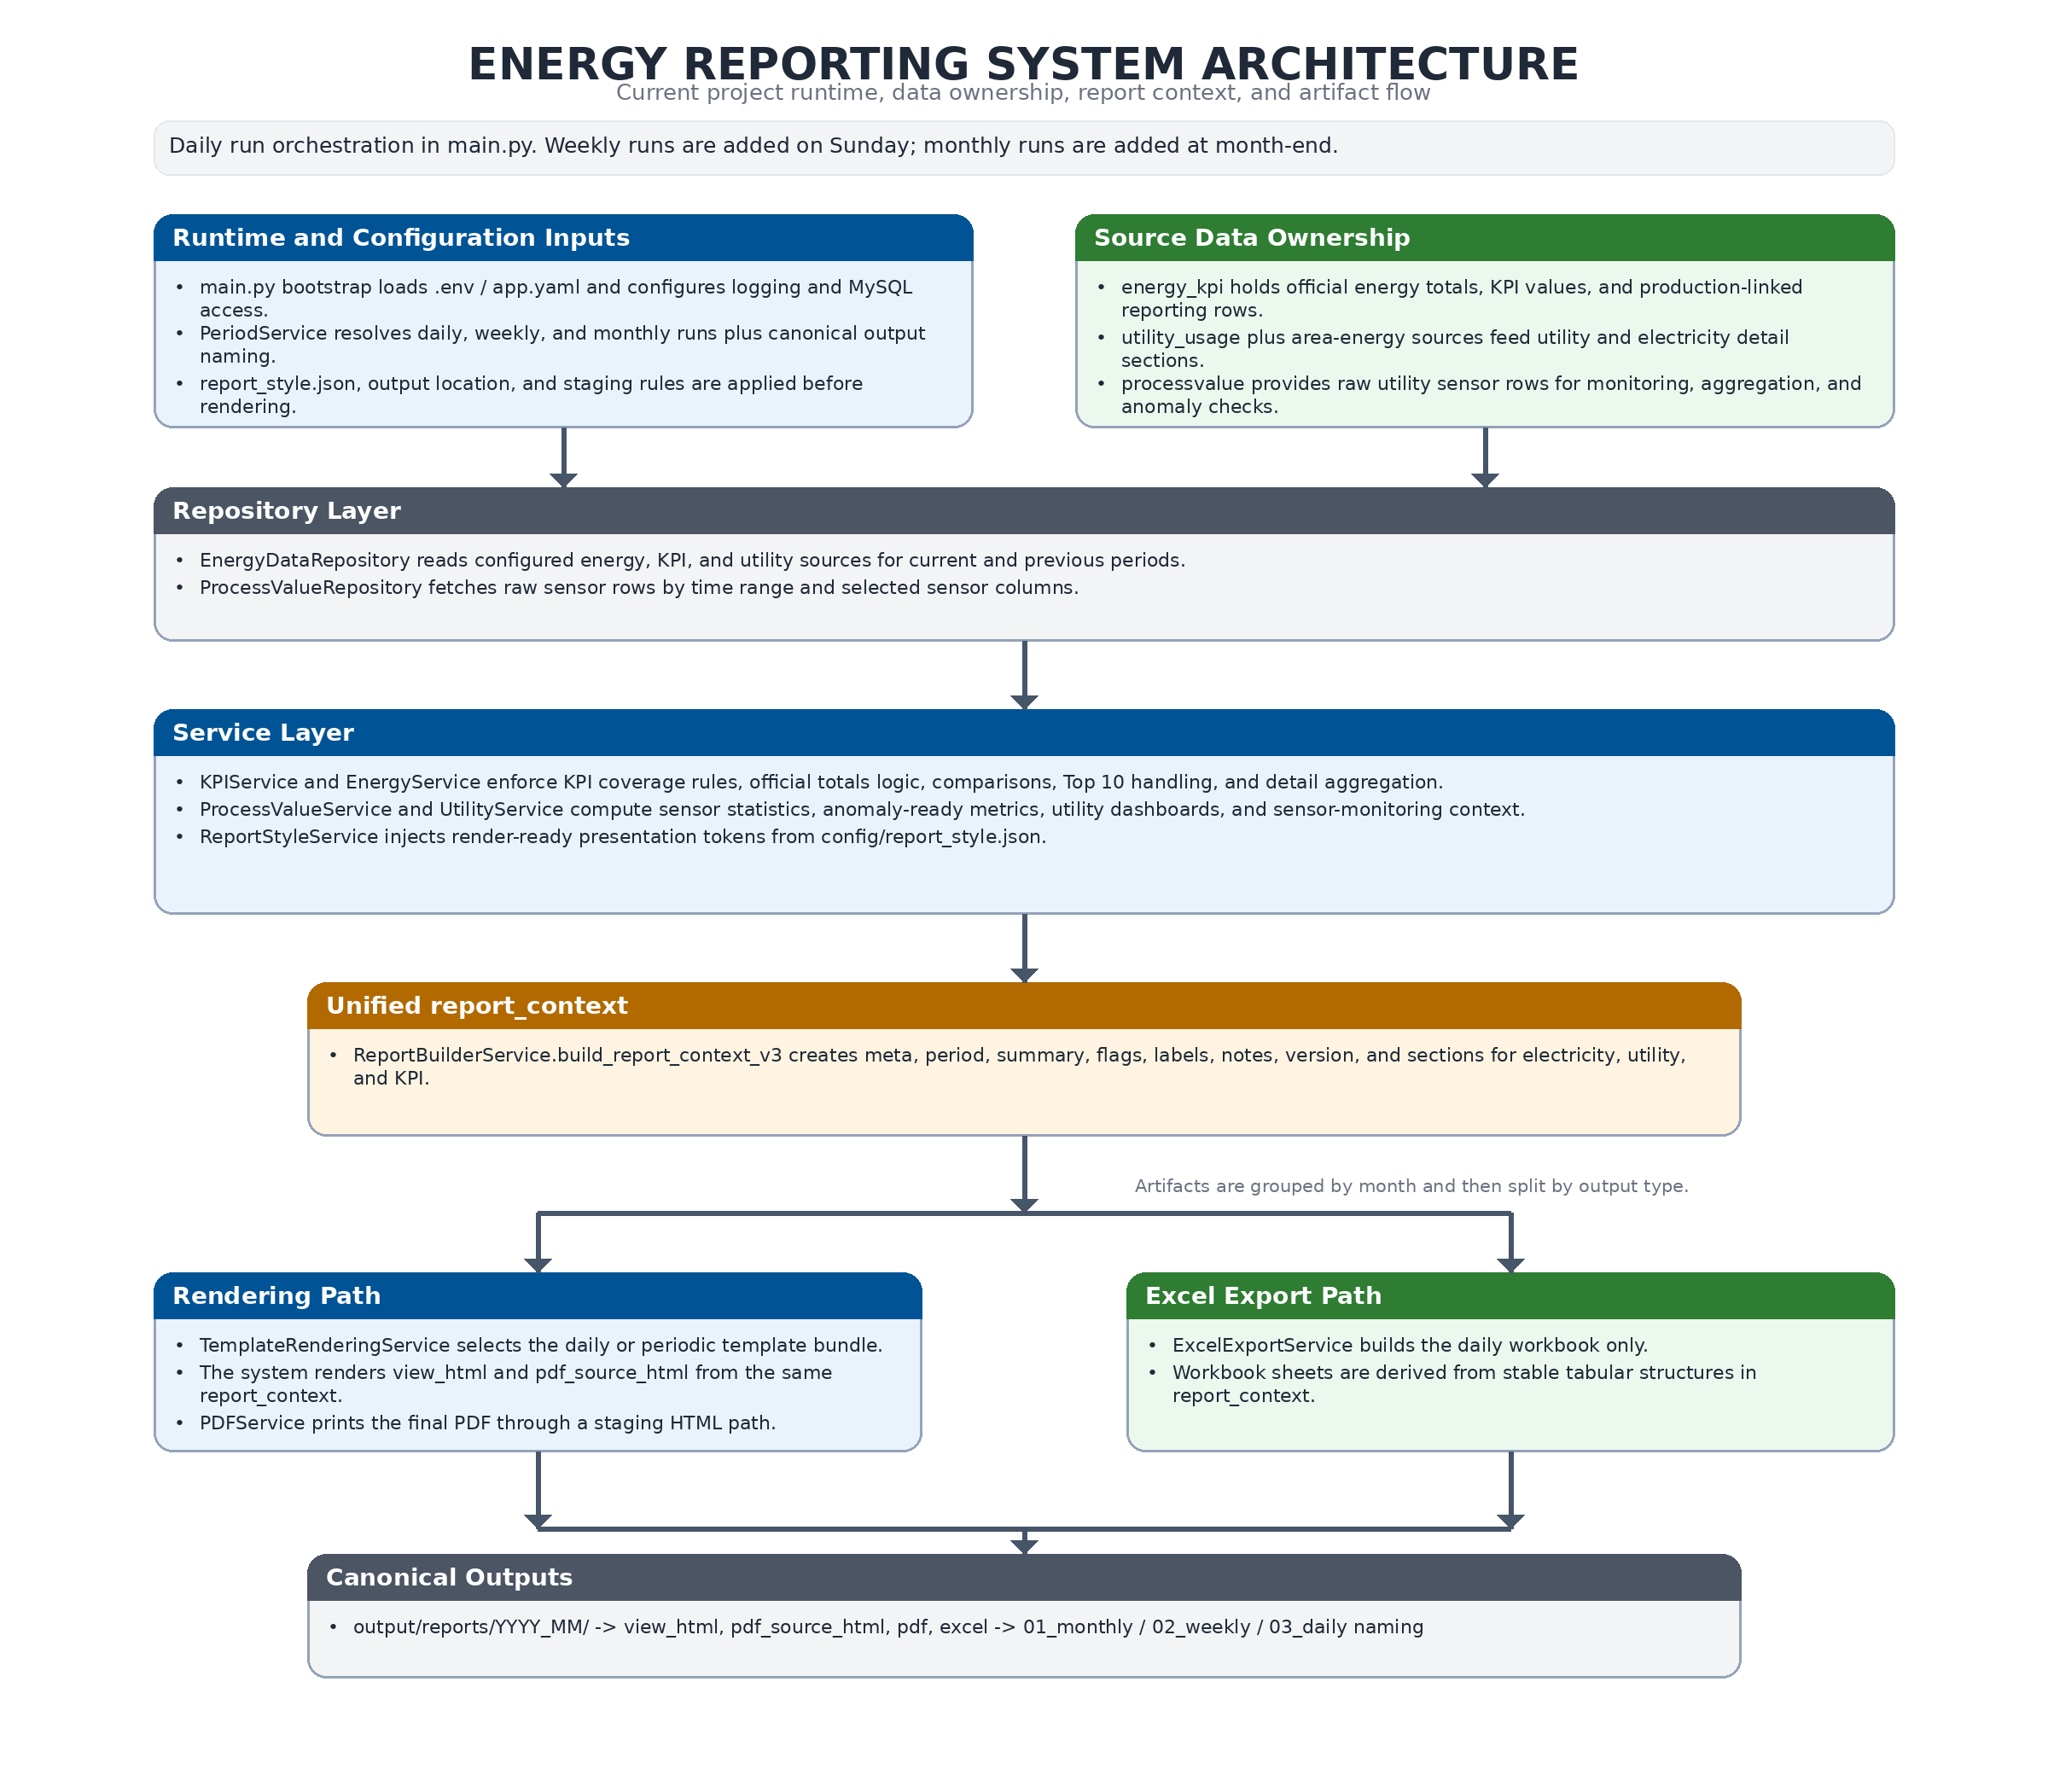
\includegraphics[width=\textwidth]{figure/hinh1_1.png}
	\caption{System architecture of the automated energy reporting pipeline}
	\label{fig:system_architecture}
\end{figure}

Hình \ref{fig:system_architecture} mô tả các lớp chính của hệ thống, bao gồm runtime/configuration inputs, data ownership, repository layer, service layer, report context builder, rendering path, Excel export path, và canonical output structure.

\begin{figure}[H]
	\centering
	% Draw.io source: figure/project_diagrams.drawio, sheet "Report Generation Flow".
	% Export artifact: figure/hinh1_2.png.
	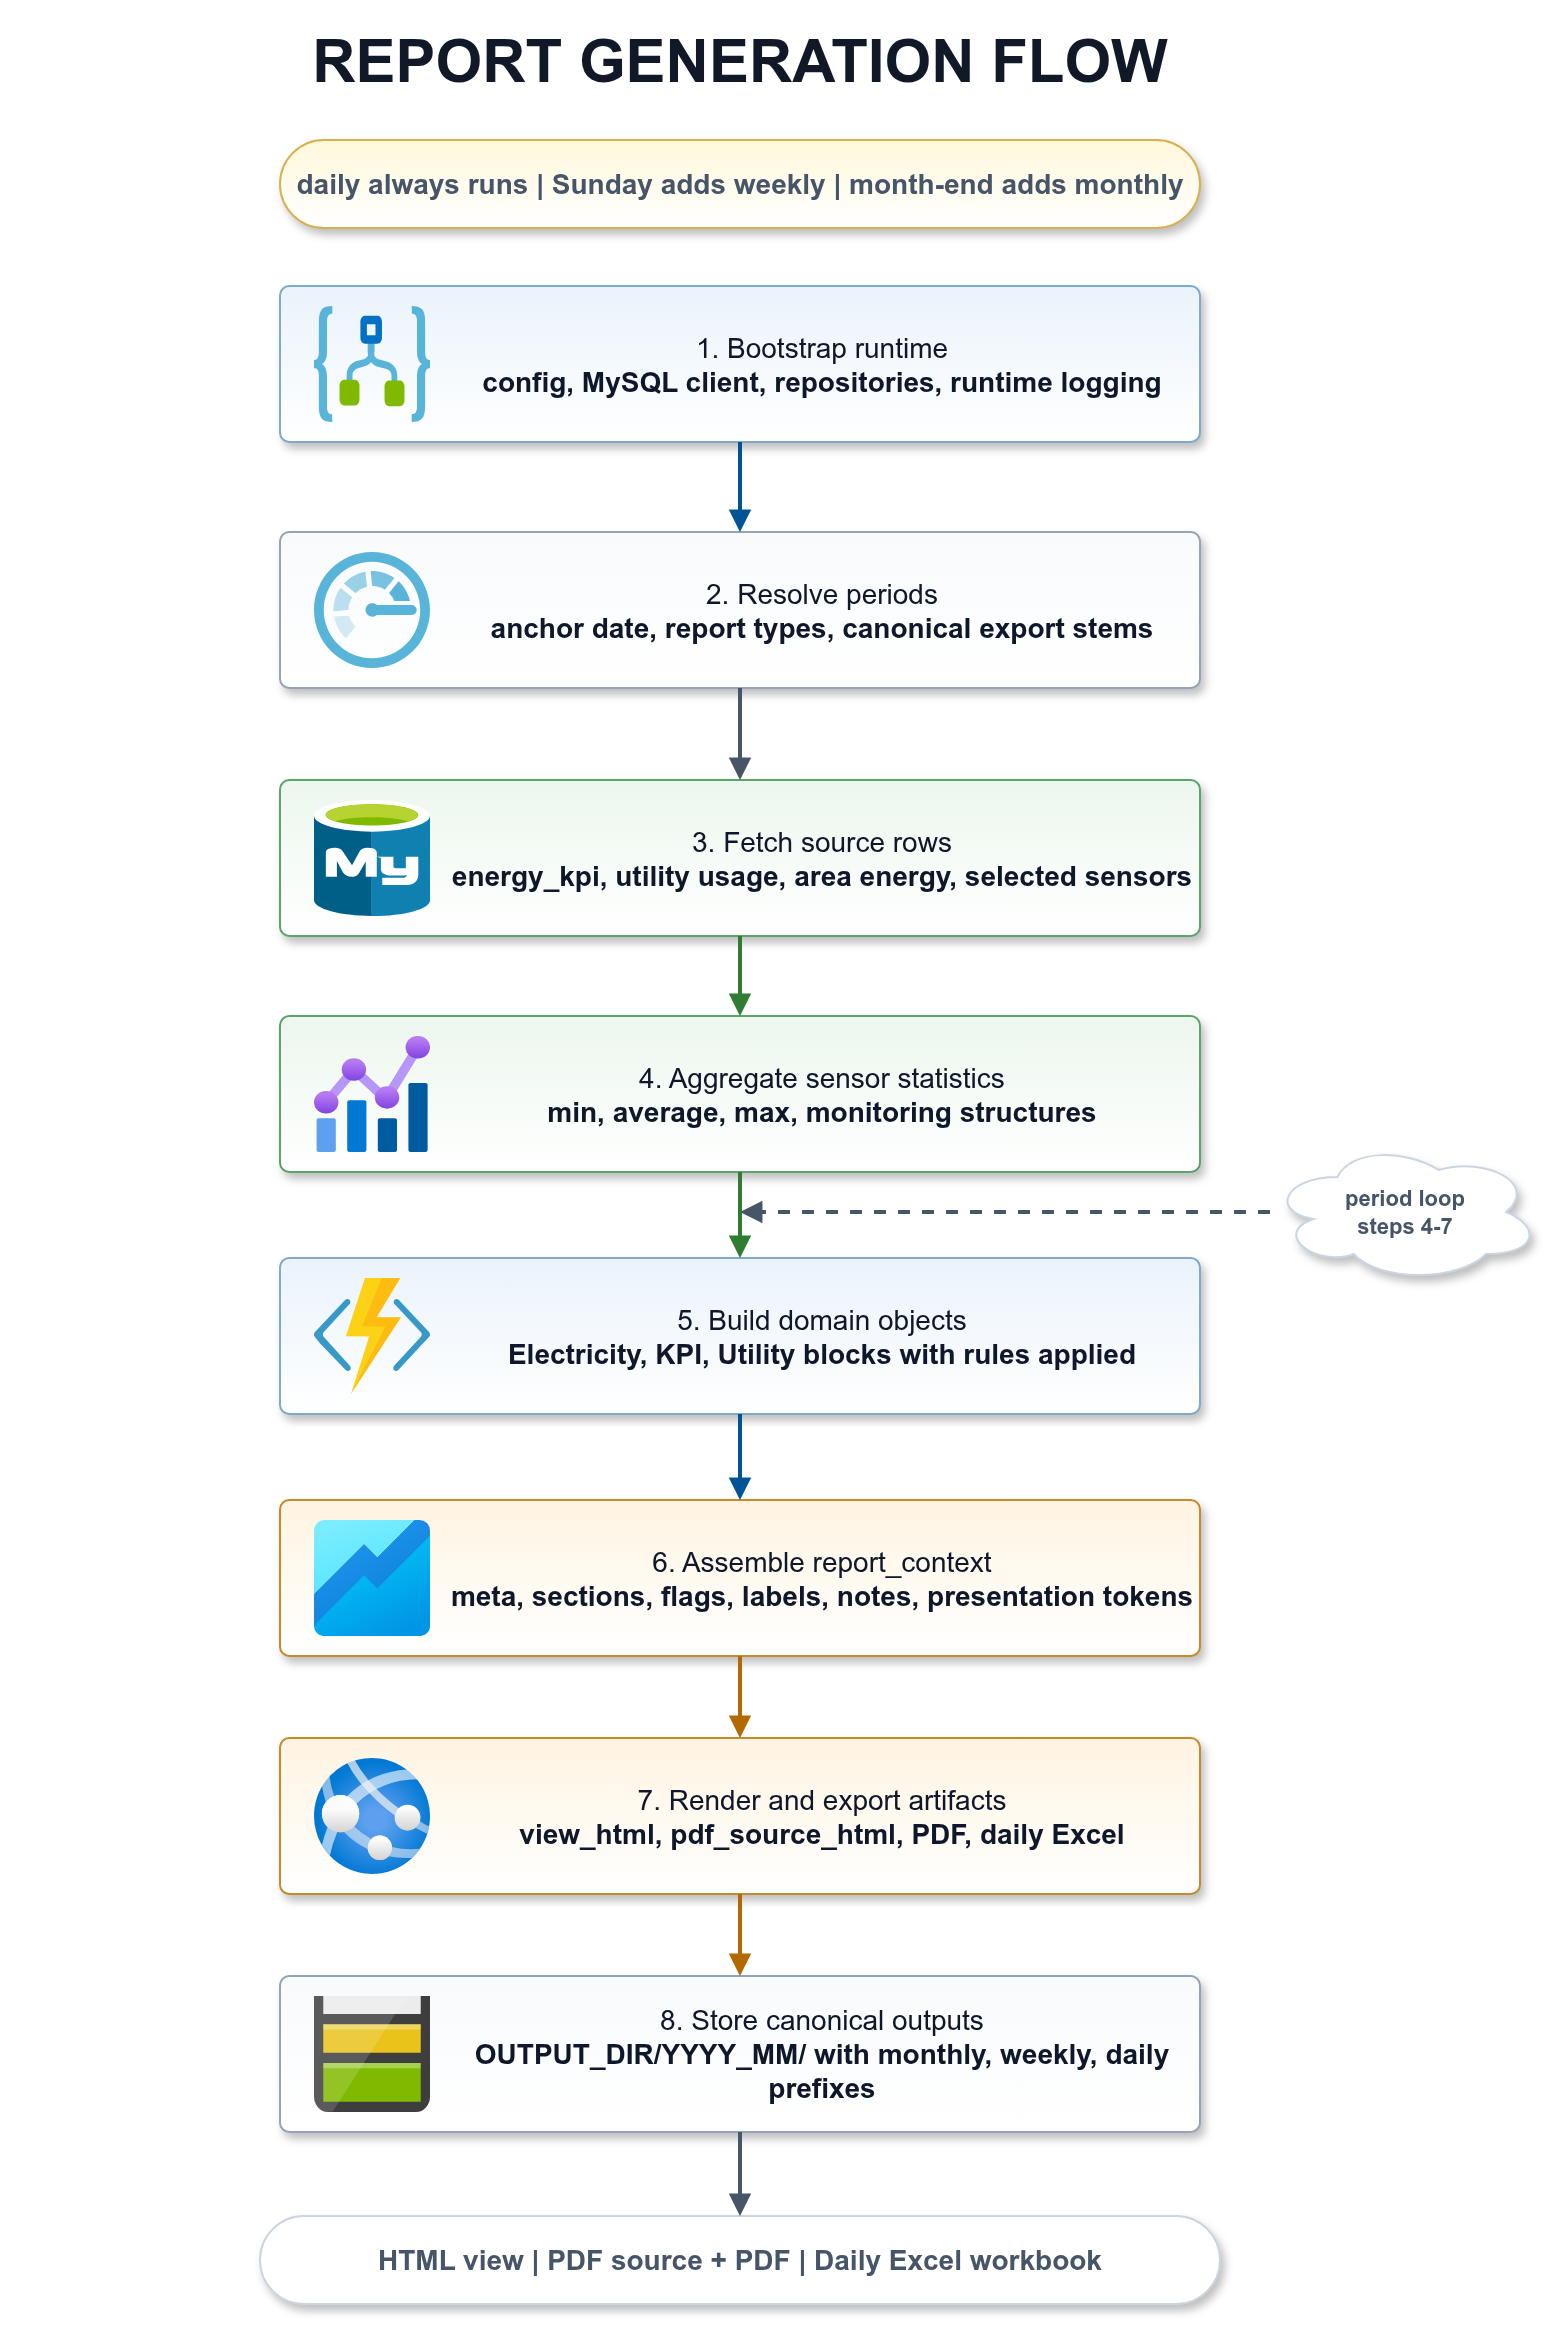
\includegraphics[width=\textwidth]{figure/hinh1_2.png}
	\caption{Report generation and export data flow for the current project runtime}
	\label{fig:report_generation_flow}
\end{figure}

Hình \ref{fig:report_generation_flow} mô tả chu trình thực thi từ bước load config, resolve scheduled periods, fetch source rows, aggregate sensor statistics, build domain objects, assemble \texttt{report\_context}, render artifacts, đến lưu output theo cấu trúc tháng.

\clearpage

\section{Ma trận thành phần chính}

Bảng \ref{tab:component_matrix} là ví dụ về cách trình bày một bảng kỹ thuật ngắn gọn, tập trung vào trách nhiệm chính và output của từng domain.

\begin{table}[htbp]
	\centering
	\renewcommand{\arraystretch}{1.3}
	\caption{Project component matrix for the energy reporting system}
	\label{tab:component_matrix}
	\begin{tabularx}{\linewidth}{|>{\RaggedRight\arraybackslash}p{3.0cm}|>{\RaggedRight\arraybackslash}X|>{\RaggedRight\arraybackslash}X|}
		\hline
		\textbf{Component} & \textbf{Primary Responsibility} & \textbf{Typical Output} \\ \hline
		Electricity domain & Official totals, area totals, comparison blocks, Top 10 meters, and detail tables & HTML sections, PDF sections, Excel detail sheets \\ \hline
		Utility domain & Utility consumption, utility energy, sensor monitoring, and anomaly-ready summaries & HTML/PDF tables, sensor monitoring cards, Excel utility sheets \\ \hline
		KPI domain & Coverage-first KPI context, production linkage, variance analysis, and comparison charts & KPI summary cards, matrices, detail blocks, charts \\ \hline
		Export workflow & Render view HTML, PDF source HTML, PDF, and daily Excel workbook with canonical naming & Month-grouped output artifacts under the project output tree \\ \hline
		Documentation workflow & Maintain project technical documentation, rebuild PDF when docs change, and preserve release-ready references & Versioned technical PDF under \texttt{docs/output/} \\ \hline
	\end{tabularx}
\end{table}

\section{Quy tắc nghiệp vụ và nguyên tắc tính toán}

Các tài liệu kỹ thuật trong dự án nên mô tả rõ các nguyên tắc cốt lõi sau:

\begin{enumerate}[label=-]
\item \textbf{Source of truth}: \texttt{energy\_kpi} là nguồn chính thức cho KPI reporting và official energy totals.
\item \textbf{Coverage-first KPI logic}: không prorate KPI blocks và luôn ưu tiên kỳ có coverage hợp lệ.
\item \textbf{Missing vs zero}: giá trị bằng 0 là dữ liệu hợp lệ, còn dữ liệu thiếu phải được thể hiện rõ ràng.
\item \textbf{Dense period rendering}: các bảng theo ngày hoặc theo kỳ phải render đủ các mốc cần thiết, không bỏ sót hàng chỉ vì thiếu giá trị.
\item \textbf{Backend-first business logic}: business rules nằm ở service/backend layer, không nhân bản logic trong template.
\item \textbf{Output consistency}: view HTML, PDF source HTML, PDF, và Excel phải bám cùng report context và cùng naming convention đã được chấp nhận.
\end{enumerate}

Các nguyên tắc vận hành năng lượng và quản lý hệ thống năng lượng như ISO 50001 là nguồn tham chiếu phù hợp khi xây dựng các mô tả ở mức policy hoặc quản trị tổng thể \cite{ref_iso50001}.

\section{Ví dụ công thức KPI}

Một ví dụ đơn giản nhưng sát ngữ cảnh dự án là công thức intensity-based KPI:

\begin{equation}
	\text{Energy Intensity} = \frac{\text{Total Energy Consumption}}{\text{Production Output}}
	\label{eq:energy_intensity}
\end{equation}

Công thức \ref{eq:energy_intensity} nên chỉ được áp dụng khi cả hai thành phần năng lượng và sản lượng đều có coverage hợp lệ và đáp ứng business rule của kỳ báo cáo.

\begin{tabular}{|p{0.5cm}|l|l|}
	\hline
	& $\text{Total Energy Consumption}$ &: Tổng năng lượng của kỳ báo cáo;\\ \hline
	& $\text{Production Output}$ &: Sản lượng hợp lệ của cùng kỳ;\\ \hline
	& $\text{Energy Intensity}$ &: Chỉ số năng lượng trên đơn vị sản lượng.\\ \hline
\end{tabular}

Khi tài liệu mô tả các công thức cụ thể hơn, nên nêu kèm điều kiện áp dụng, quy tắc coverage, và các trường hợp không được tính để tránh hiểu sai logic implementation.

\section{Workflow cập nhật tài liệu và phát hành PDF}

Workflow khuyến nghị cho subsystem tài liệu kỹ thuật là:

\begin{enumerate}[label=-]
\item cập nhật source Markdown hoặc LaTeX liên quan đến project documentation;
\item kiểm tra lại hình, biểu đồ, tài liệu tham khảo, và các file \texttt{\textbackslash input};
\item build lại PDF bằng \texttt{latexmk + XeLaTeX + biber};
\item kiểm tra PDF đầu ra trong \texttt{docs/output/};
\item chỉ phát hành hoặc chia sẻ khi nội dung tài liệu khớp với trạng thái implementation và naming rules hiện tại.
\end{enumerate}

Đối với project này, PDF không cần rebuild cho mọi thay đổi code. PDF chỉ cần rebuild khi các source tài liệu, hình minh họa, tài liệu tham khảo, hoặc workflow/rules của documentation thay đổi. Cách tiếp cận này phù hợp với mục tiêu giữ tài liệu luôn đồng bộ mà không tạo thêm noise không cần thiết trong pipeline vận hành.

\section{Kiểm soát thay đổi và checklist phát hành}

Trước khi phát hành một bản technical PDF mới, nên rà soát tối thiểu các hạng mục sau:

\begin{enumerate}[label=-]
\item tên tài liệu, phạm vi, và phiên bản tài liệu;
\item tính nhất quán giữa nội dung mô tả và code hiện tại;
\item tính đúng đắn của business rules và KPI calculation notes;
\item tính hợp lệ của figures, tables, cross references, và bibliography;
\item output naming và vị trí lưu file PDF;
\item việc có hay không cần cập nhật checklist, runbook, hoặc project status song song với tài liệu PDF.
\end{enumerate}

\section{Current handover-readiness snapshot}

Ở trạng thái hiện tại, bộ technical manual đã có một cấu trúc đủ rõ để dùng cho internal handover review. Chapter order hiện hành gồm:

\begin{enumerate}[label=-]
\item document metadata và revision history;
\item project overview và phạm vi tài liệu;
\item data sources và repository / service mapping;
\item business rules và KPI reporting rules;
\item output structure và release workflow;
\item deployment and operations;
\item troubleshooting;
\item glossary và naming conventions dưới dạng appendix.
\end{enumerate}

Các thành phần trên đã tạo được một luồng đọc hợp lý từ governance, sang architecture, data ownership, business rules, vận hành, và cuối cùng là lớp tra cứu thuật ngữ. Điều này phù hợp với mục tiêu dùng bộ PDF như một tài liệu kỹ thuật có thể review, handover, và đối chiếu với runtime thật.

Ở góc nhìn readiness, các điểm đã đủ tốt cho internal review gồm:

\begin{enumerate}[label=-]
\item chapter order đã ổn định và không còn mang tính lecture-template;
\item glossary appendix đã tồn tại thật, không còn ở trạng thái placeholder;
\item revision history đã phản ánh các checkpoint chính của subsystem LaTeX;
\item output structure, deployment baseline, naming conventions, và PDF rebuild rules đã được mô tả rõ;
\item generated technical PDFs đã được rebuild và verify sau các lần cập nhật chính.
\end{enumerate}

Các điểm còn mở trước khi xem tài liệu là approved handover baseline gồm:

\begin{enumerate}[label=-]
\item gán reviewer chính thức cho bản technical manual;
\item chốt approver hoặc sign-off owner;
\item sau vòng review nội bộ, cân nhắc freeze một version ổn định hơn như \texttt{v1.0} nếu không còn thay đổi lớn về cấu trúc.
\end{enumerate}

\section{Documentation maintenance checklist}

Checklist tối thiểu để duy trì bộ tài liệu ở trạng thái usable và không drift khỏi implementation là:

\begin{enumerate}[label=-]
\item xác nhận phạm vi update của tài liệu;
\item xác nhận các screenshot, sơ đồ, bảng biểu, và examples phản ánh đúng implementation hiện tại;
\item rà lại business rules, KPI formulas, output naming, và source-of-truth notes nếu thay đổi có chạm vào domain logic;
\item build lại PDF và kiểm tra \texttt{docs/output/} khi documentation source, figures, references, hoặc workflow rules thay đổi;
\item chỉ chia sẻ hoặc dùng cho review khi nội dung và formatting đã được rà lại đầy đủ.
\end{enumerate}

\noindent\textbf{Operational notes}

\begin{enumerate}[label=-]
\item Technical documentation phải được cập nhật khi docs source thay đổi có ý nghĩa, không để trôi xa implementation.
\item Generated PDFs là output artifacts, không phải primary source.
\item Nếu build lỗi, cần giữ log và báo lỗi rõ thay vì bỏ qua bước rebuild hoặc review PDF.
\end{enumerate}

\section{Tổng kết chương}

Chapter tổng quan này hiện không còn là một chapter mẫu thuần túy. Nó đã trở thành phần mở đầu thực sự của bộ technical manual, mô tả mục tiêu tài liệu, phạm vi, kiến trúc hệ thống, workflow cập nhật docs, và trạng thái handover-readiness hiện tại. Kết hợp với các chapter còn lại và appendix glossary, bộ tài liệu hiện đã ở mức phù hợp cho internal review và gần sẵn sàng cho một baseline handover có kiểm soát.

	\chapter{DATA SOURCES VÀ REPOSITORY / SERVICE MAPPING}

\begin{ChapterObjectives}
\item Mô tả rõ các data sources cốt lõi đang nuôi hệ thống báo cáo năng lượng.
\item Ghi nhận repository nào đọc từng source và service nào chịu trách nhiệm diễn giải dữ liệu đó.
\item Tạo một ownership map giữa database layer, repository layer, service layer, và report context builder.
\item Giúp người phát triển mới hoặc người bàn giao có thể lần theo luồng dữ liệu từ bảng nguồn đến artifact cuối cùng.
\end{ChapterObjectives}

\section{Vai trò của chapter data sources và mapping}

Trong một hệ thống reporting hoặc ETL, việc hiểu đúng data ownership quan trọng không kém việc hiểu đúng business rules. Nếu business rules trả lời câu hỏi \textit{dữ liệu phải được dùng như thế nào}, thì chapter mapping này trả lời câu hỏi \textit{dữ liệu đang đi từ đâu đến đâu, và lớp nào chịu trách nhiệm cho mỗi bước}. Đây là nền tảng giúp người đọc đối chiếu tài liệu với codebase thực tế và giảm rủi ro sửa sai tầng logic \cite{ref_kimball,ref_mysql,ref_python}.

Đối với dự án này, luồng chuẩn cần được hiểu theo các lớp sau:

\begin{enumerate}[label=-]
\item database objects và raw source tables/views;
\item repositories chịu trách nhiệm query và trả về raw structured rows;
\item services chịu trách nhiệm áp dụng rule, aggregate, và chuẩn hóa thành domain objects;
\item report context builder chịu trách nhiệm hợp nhất các domain objects vào một \texttt{report\_context};
\item rendering/export layer chuyển \texttt{report\_context} thành HTML, PDF, và Excel artifacts.
\end{enumerate}

\section{Primary data sources}

\subsection{Configured logical datasets}

Module \texttt{src/config/data\_sources.py} hiện cấu hình các logical dataset sau:

\begin{enumerate}[label=-]
\item \texttt{all\_energy}
\item \texttt{diode\_energy}
\item \texttt{ico\_energy}
\item \texttt{sakari\_energy}
\item \texttt{utility\_usage}
\item \texttt{energy\_kpi}
\end{enumerate}

Trong số này, \texttt{diode\_energy}, \texttt{ico\_energy}, và \texttt{sakari\_energy} là các view phục vụ electricity detail và comparison theo area. \texttt{utility\_usage} là view phục vụ Utility reporting. \texttt{energy\_kpi} là table đặc biệt vì nó mang vai trò source-of-truth cho KPI reporting và official totals.

\subsection{Source-of-truth tables and views}

Bảng \ref{tab:data_source_inventory} tóm tắt inventory nguồn dữ liệu hiện hành theo góc nhìn kỹ thuật.

\begin{table}[htbp]
	\centering
	\renewcommand{\arraystretch}{1.3}
	\caption{Configured data source inventory}
	\label{tab:data_source_inventory}
	\begin{tabularx}{\linewidth}{|>{\RaggedRight\arraybackslash}p{2.8cm}|>{\RaggedRight\arraybackslash}p{2.1cm}|>{\RaggedRight\arraybackslash}p{2.0cm}|>{\RaggedRight\arraybackslash}X|}
		\hline
		\textbf{Logical Dataset} & \textbf{Object Type} & \textbf{Date Column} & \textbf{Primary Use} \\ \hline
		\texttt{all\_energy} & view & \texttt{dt} & nguồn tổng quát cho energy-related exploration hoặc future aggregation slices. \\ \hline
		\texttt{diode\_energy} & view & \texttt{dt} & chi tiết điện năng theo area DIODE. \\ \hline
		\texttt{ico\_energy} & view & \texttt{dt} & chi tiết điện năng theo area ICO. \\ \hline
		\texttt{sakari\_energy} & view & \texttt{dt} & chi tiết điện năng theo area SAKARI. \\ \hline
		\texttt{utility\_usage} & view & \texttt{dt} & utility daily detail, utility summary, và utility comparison blocks. \\ \hline
		\texttt{energy\_kpi} & table & none at config level & source-of-truth cho KPI rows, official totals, production values, và energy-linked KPI reporting. \\ \hline
		\texttt{processvalue} & raw table & \texttt{Time\_Stamp} & raw utility sensor rows cho sensor monitoring, anomaly-ready aggregation, và trend context. \\ \hline
	\end{tabularx}
\end{table}

\subsection{Energy KPI as authoritative source}

\texttt{energy\_kpi} là nguồn quan trọng nhất về mặt nghiệp vụ. Table này không chỉ chứa KPI values mà còn chứa official plant totals, official area totals, production context, và các stored blocks cần cho KPI coverage logic. Chính vì vậy:

\begin{enumerate}[label=-]
\item Electricity official totals phải dựa trên \texttt{energy\_kpi};
\item KPI reporting phải dựa trên \texttt{energy\_kpi};
\item production-linked reporting cũng phải tham chiếu \texttt{energy\_kpi};
\item không được tự reconstruct hoặc recompute KPI từ raw energy views nếu rule không cho phép.
\end{enumerate}

\subsection{Processvalue as raw sensor source}

\texttt{processvalue} là raw sensor source cho utility sensor monitoring. Bảng này được đọc ở granularity timestamped rows và sau đó mới được aggregate thành daily sensor statistics. Điều đó có nghĩa là \texttt{processvalue} không phải business-ready surface; nó là nguồn thô cho một nhánh xử lý riêng trước khi dữ liệu được đưa vào \texttt{report\_context}.

\section{Repository layer mapping}

\subsection{EnergyDataRepository}

\texttt{EnergyDataRepository} là repository tổng quát dùng cho các energy-like tabular sources. Repository này chịu trách nhiệm:

\begin{enumerate}[label=-]
\item validate source configuration;
\item introspect metadata columns qua \texttt{INFORMATION\_SCHEMA};
\item xác định meter columns hợp lệ dựa trên numeric MySQL types;
\item truy vấn daily detail rows;
\item truy vấn meter totals hoặc top-N related aggregations cho các sources có cấu trúc dạng energy table/view.
\end{enumerate}

Điểm mạnh của repository này là không hard-code database object cụ thể vào logic query. Thay vào đó, nó nhận \texttt{DataSourceConfig} và dùng cùng một abstraction cho nhiều logical datasets khác nhau.

\subsection{ProcessValueRepository}

\texttt{ProcessValueRepository} có phạm vi hẹp hơn nhưng rõ ràng hơn. Repository này chỉ làm một việc chính: đọc raw sensor rows từ \texttt{ems\_db.processvalue}. Nó:

\begin{enumerate}[label=-]
\item nhận khoảng thời gian \texttt{start\_dt} và \texttt{end\_dt\_exclusive};
\item nhận danh sách sensor columns cần chọn;
\item build SELECT an toàn cho \texttt{Time\_Stamp} cộng các sensor columns;
\item trả về danh sách rows theo format chuẩn có khóa \texttt{dt}.
\end{enumerate}

Repository này không aggregate, không format, và không áp business rules. Điều đó giữ cho raw sensor access đơn giản và dễ test.

\subsection{Repository ownership matrix}

Bảng \ref{tab:repository_mapping} tóm tắt mapping giữa data sources và repository ownership.

\begin{table}[htbp]
	\centering
	\renewcommand{\arraystretch}{1.3}
	\caption{Repository ownership mapping}
	\label{tab:repository_mapping}
	\begin{tabularx}{\linewidth}{|>{\RaggedRight\arraybackslash}p{3.0cm}|>{\RaggedRight\arraybackslash}p{3.3cm}|>{\RaggedRight\arraybackslash}X|}
		\hline
		\textbf{Source} & \textbf{Repository Owner} & \textbf{Repository Responsibility} \\ \hline
		\texttt{diode\_energy}, \texttt{ico\_energy}, \texttt{sakari\_energy}, \texttt{utility\_usage}, \texttt{energy\_kpi} & \texttt{EnergyDataRepository} & fetch daily rows, inspect columns, expose meter columns, and provide structured tabular data for higher-level services. \\ \hline
		\texttt{processvalue} & \texttt{ProcessValueRepository} & fetch raw timestamped sensor rows for selected columns and time windows only. \\ \hline
	\end{tabularx}
\end{table}

\section{Service layer mapping}

\subsection{EnergyService}

\texttt{EnergyService} chịu trách nhiệm dựng domain object cho Electricity. Nó nhận area rows, area columns, KPI-linked summary inputs, và trả ra các nhóm dữ liệu như:

\begin{enumerate}[label=-]
\item summary;
\item top meter comparison;
\item daily summary rows;
\item daily area tables;
\item anomalies và topology-aware diagnostics khi cần.
\end{enumerate}

Một chi tiết quan trọng là \texttt{EnergyService} không xem raw view totals là official totals. Nó sử dụng KPI-linked values làm reference cho plant total và area total theo các rule đã chốt.

\subsection{KPIService}

\texttt{KPIService} là lớp xử lý raw KPI rows trước khi chúng trở thành business-approved KPI objects. Nó chịu trách nhiệm:

\begin{enumerate}[label=-]
\item deduplicate rows theo \texttt{dt\_start}, \texttt{dt\_end}, và \texttt{time\_frame};
\item chọn row mới nhất theo \texttt{dt\_lastupdate};
\item resolve best KPI rows cho một report period theo coverage-first logic;
\item build KPI summary và daily detail surface từ các selected rows đã hợp lệ.
\end{enumerate}

Nói cách khác, \texttt{KPIService} là lớp hiện thực hóa rule Day $>$ Week $>$ Month $>$ Year, no-prorating, no-overlap, và no-reconstruction-from-raw-views.

\subsection{UtilityService}

\texttt{UtilityService} chịu trách nhiệm chuyển \texttt{utility\_usage} rows thành utility reporting object ở cấp domain. Nó:

\begin{enumerate}[label=-]
\item build utility summary;
\item build dense daily utility timeseries;
\item build current/previous comparison blocks;
\item gắn sensor monitoring context vào utility object;
\item map raw utility columns thành business-friendly metric structures.
\end{enumerate}

\subsection{ProcessValueService}

\texttt{ProcessValueService} là service aggregate dành riêng cho raw \texttt{processvalue} rows. Nó không biết gì về utility dashboard ở cấp business. Vai trò của nó là:

\begin{enumerate}[label=-]
\item gom rows theo ngày;
\item tính \texttt{min}, \texttt{avg}, \texttt{max}, \texttt{value\_sum}, \texttt{latest};
\item đếm \texttt{sample\_count}, \texttt{non\_null\_count}, \texttt{zero\_count}, \texttt{negative\_count};
\item trả về daily sensor statistics để \texttt{UtilityService} và sensor-monitoring flow có thể dùng tiếp.
\end{enumerate}

Sự tách lớp giữa \texttt{ProcessValueRepository} và \texttt{ProcessValueService} rất có giá trị vì nó giữ ranh giới rõ giữa raw data access và aggregation logic.

\subsection{Style and render-context services}

Ngoài các domain services, còn có một service đặc biệt tham gia vào report context assembly là \texttt{ReportStyleService}. Service này không xử lý dữ liệu nghiệp vụ; nó xử lý presentation tokens từ \texttt{config/report\_style.json} và merge chúng vào render context để view/PDF layers có thể dùng chung một nguồn style đã được normalize.

\section{End-to-end build mapping in main.py}

Từ góc nhìn orchestration, \texttt{src/main.py} thực hiện mapping các lớp như sau:

\begin{enumerate}[label=-]
\item \texttt{\_bootstrap()} load config, tạo MySQL client, và khởi tạo repositories từ \texttt{get\_data\_sources()};
\item \texttt{\_build\_kpi\_object()} dùng repository \texttt{energy\_kpi} và \texttt{KPIService};
\item \texttt{\_build\_sensor\_monitoring\_context()} dùng \texttt{ProcessValueRepository}, \texttt{ProcessValueService}, và \texttt{UtilityService};
\item \texttt{\_build\_utility\_object()} dùng repository \texttt{utility\_usage} và utility sensor monitoring context;
\item \texttt{\_build\_energy\_object()} dùng area energy repositories cộng KPI-linked summary inputs;
\item \texttt{\_build\_report\_context()} dùng \texttt{ReportBuilderService} và \texttt{ReportStyleService};
\item \texttt{\_render\_report\_artifacts()} dùng \texttt{TemplateRenderingService}, \texttt{PDFService}, và \texttt{ExcelExportService} để sinh output artifacts.
\end{enumerate}

Công thức lineage ngắn gọn của dự án có thể được mô tả như sau:

\begin{equation}
	\text{Database Sources} \rightarrow \text{Repositories} \rightarrow \text{Services} \rightarrow \text{report\_context} \rightarrow \text{HTML / PDF / Excel Artifacts}
	\label{eq:data_lineage}
\end{equation}

\section{Ownership map by domain}

Bảng \ref{tab:domain_owner_map} tổng hợp ownership ở cấp domain và execution flow.

\begin{table}[htbp]
	\centering
	\renewcommand{\arraystretch}{1.3}
	\caption{Domain owner map from source to output}
	\label{tab:domain_owner_map}
	\begin{tabularx}{\linewidth}{|>{\RaggedRight\arraybackslash}p{2.1cm}|>{\RaggedRight\arraybackslash}p{2.6cm}|>{\RaggedRight\arraybackslash}p{2.8cm}|>{\RaggedRight\arraybackslash}X|}
		\hline
		\textbf{Domain} & \textbf{Primary Source} & \textbf{Repository / Service Path} & \textbf{Output Contribution} \\ \hline
		Electricity & area energy views + \texttt{energy\_kpi} & \shortstack[l]{\texttt{EnergyDataRepository} \\ $\rightarrow$ \texttt{EnergyService}} & electricity summary cards, top meter tables, daily detail tables, comparison blocks \\ \hline
		KPI & \texttt{energy\_kpi} & \shortstack[l]{\texttt{EnergyDataRepository} \\ $\rightarrow$ \texttt{KPIService}} & KPI summary, coverage notes, daily KPI detail, comparison surfaces \\ \hline
		Utility usage & \texttt{utility\_usage} & \shortstack[l]{\texttt{EnergyDataRepository} \\ $\rightarrow$ \texttt{UtilityService}} & utility summary, dense utility tables, utility comparison blocks \\ \hline
		Sensor monitoring & \texttt{processvalue} + sensor metadata & \shortstack[l]{\texttt{ProcessValueRepository} \\ $\rightarrow$ \texttt{ProcessValueService} \\ $\rightarrow$ \texttt{UtilityService}} & sensor overview cards, daily sensor rows, anomaly-ready payloads, periodic detail tables \\ \hline
		Rendering context & \texttt{report\_style.json} + domain objects & \shortstack[l]{\texttt{ReportStyleService} \\ + \texttt{ReportBuilderService}} & unified render-ready context for HTML/PDF templates \\ \hline
	\end{tabularx}
\end{table}

\section{Implementation guardrails for future changes}

Khi thay đổi một source hoặc một service, nên giữ các guardrail sau:

\begin{enumerate}[label=-]
\item nếu một metric đang lấy từ \texttt{energy\_kpi}, không được tự chuyển sang raw view chỉ để tiện implementation;
\item nếu một repository chỉ chịu trách nhiệm fetch raw rows, không đẩy business logic xuống repository layer;
\item nếu một service đang aggregate hoặc resolve coverage, không dời logic đó xuống template;
\item nếu thay đổi metadata mappings hoặc sensor columns, phải rà lại impact lên cả utility object và sensor monitoring payload;
\item nếu thay đổi context structure, phải rà lại HTML view, PDF source HTML, PDF render, và Excel export cùng lúc;
\item docs của technical manual phải được cập nhật song song khi ownership map hoặc data lineage thay đổi đáng kể.
\end{enumerate}

\section{Tổng kết chương}

Chapter này xác định rõ data lineage của hệ thống: từ các nguồn \texttt{energy\_kpi}, energy views, \texttt{utility\_usage}, và \texttt{processvalue}; qua các repositories và services tương ứng; đến \texttt{report\_context} và các artifacts cuối cùng. Sau chapter này, bộ technical manual đã có thêm lớp mô tả rất quan trọng để người đọc hiểu không chỉ \textit{rule gì đang áp dụng}, mà còn \textit{dữ liệu đi qua những lớp nào trước khi thành báo cáo}. 

	\chapter{BUSINESS RULES VÀ KPI REPORTING RULES}

\noindent\textbf{Mục tiêu chương}

\begin{enumerate}[label=-]
\item Tóm tắt các business rules cốt lõi đang chi phối hệ thống báo cáo năng lượng.
\item Ghi nhận rõ source-of-truth rules, period rules, display rules, và KPI coverage rules.
\item Giúp kỹ sư phát triển, người rà soát nghiệp vụ, và người vận hành có cùng cách hiểu về logic hiện hành.
\item Tạo một chapter chuẩn để mở rộng thành tài liệu rules chính thức khi dự án tiếp tục hoàn thiện.
\end{enumerate}

\section{Vai trò của business rules trong dự án}

Đối với hệ thống báo cáo năng lượng, business rules không chỉ quyết định cách hiển thị báo cáo mà còn quyết định cách dữ liệu được chọn, được tổng hợp, và được chấp nhận để phát hành. Các rule được mô tả trong chapter này phải luôn bám sát implementation thực tế và nhất quán với các tài liệu nguồn như \texttt{docs/business\_rules.md} và \texttt{docs/kpi\_reporting\_rules.md}.

Trong các hệ thống ETL hoặc reporting pipeline, việc duy trì đúng grain của dữ liệu, đúng source-of-truth, và đúng điều kiện tổng hợp là điều kiện tiên quyết để tránh sai lệch kết quả \cite{ref_kimball}. Với dự án này, phần rules là lớp bảo vệ quan trọng cho tính đúng đắn của output cuối cùng.

\section{General reporting invariants}

Các quy tắc tổng quát sau áp dụng cho toàn bộ report stack:

\begin{enumerate}[label=-]
\item báo cáo được tổ chức thành các section có cấu trúc rõ ràng, tối thiểu gồm Electricity, Utility, KPI, và phần metadata liên quan;
\item mỗi report phải hỗ trợ so sánh giữa kỳ hiện tại và kỳ trước tương ứng;
\item runtime hiện tại phát hành các kỳ \textit{daily}, \textit{weekly}, và \textit{monthly}; rules nền vẫn phải tương thích với các custom range trong tương lai nếu chúng được bật lại;
\item các bảng daily phải luôn dense, không bỏ mất ngày chỉ vì thiếu dữ liệu;
\item giá trị bằng 0 là hợp lệ, còn giá trị thiếu phải hiển thị rõ bằng dấu \texttt{-};
\item logic nghiệp vụ phải nằm ở backend/service layer, không nhân bản trong template HTML hay PDF.
\end{enumerate}

Đối với mọi metric có so sánh, backend cần chuẩn bị đầy đủ current value, previous value, delta, và delta percentage theo công thức sau:

\begin{equation}
	\Delta = \text{Current Value} - \text{Previous Value}
	\label{eq:delta_value}
\end{equation}

\begin{equation}
	\Delta\% = \begin{cases}
		\frac{\Delta}{\text{Previous Value}} \times 100, & \text{khi Previous Value} \neq 0 \\
		\texttt{-}, & \text{khi Previous Value} = 0
	\end{cases}
	\label{eq:delta_pct}
\end{equation}

Cách xử lý này giúp report phản ánh trung thực sự thay đổi mà không tạo ra phần trăm ảo trong trường hợp mẫu số bằng 0.

\section{Source of truth và ownership map}

Bảng \ref{tab:rule_ownership_matrix} tóm tắt nguồn dữ liệu chính thức và lớp chịu trách nhiệm diễn giải chúng.

\begin{table}[h]
	\centering
	\renewcommand{\arraystretch}{1.3}
	\caption{Rule ownership and source-of-truth matrix}
	\label{tab:rule_ownership_matrix}
	\begin{tabularx}{\linewidth}{|>{\RaggedRight\arraybackslash}p{3.1cm}|>{\RaggedRight\arraybackslash}p{3.2cm}|>{\RaggedRight\arraybackslash}X|}
		\hline
		\textbf{Domain} & \textbf{Primary Source / Owner} & \textbf{Critical Rule} \\ \hline
		Electricity official totals & \texttt{energy\_kpi} & Plant totals và area official totals phải dùng giá trị đã được phê duyệt, không tự cộng lại từ raw energy views. \\ \hline
		KPI values and production-linked reporting & \texttt{energy\_kpi} & KPI reporting chỉ dùng các block đã tính sẵn và đã được lưu, tuân thủ coverage-first logic. \\ \hline
		Utility daily usage & utility usage source & Utility summary và daily detail phải so sánh current/previous và giữ dense rows cho khoảng ngày cần hiển thị. \\ \hline
		Sensor monitoring & \texttt{processvalue} + sensor metadata mapping & Raw sensor rows phải được aggregate thành payload có chất lượng dữ liệu rõ ràng, hỗ trợ anomaly-ready analysis. \\ \hline
		Presentation rules & backend services + render context & Template chỉ nhận dữ liệu đã chuẩn hóa từ \texttt{report\_context}; không tái tính nghiệp vụ trong view/PDF. \\ \hline
	\end{tabularx}
\end{table}

Source-of-truth discipline này rất quan trọng vì nếu sai nguồn dữ liệu hoặc sai grain tổng hợp, toàn bộ report có thể trở nên nhất quán về hình thức nhưng sai về bản chất. Đây cũng là nguyên tắc nền trong các hệ thống dữ liệu định hướng báo cáo và warehouse \cite{ref_kimball,ref_mysql}.

\section{Electricity rules}

\subsection{Official totals và residual load}

Các rule điện năng cốt lõi gồm:

\begin{enumerate}[label=-]
\item official plant total và official area total phải lấy từ \texttt{energy\_kpi};
\item không được suy ra official totals bằng cách cộng toàn bộ meter values từ energy views, vì các energy views có thể chứa main feeders và downstream overlap;
\item main feeder definitions và area topology phải được quản lý qua metadata cấu hình của dự án;
\item residual load được xem như một virtual meter khi có đủ điều kiện tính hợp lệ.
\end{enumerate}

Residual load được định nghĩa như sau:

\begin{equation}
	\text{Residual Load} = \text{Official Area Total} - \sum \text{Branch Meters (excluding main feeders)}
	\label{eq:residual_load}
\end{equation}

Residual load đại diện cho phần tải chưa được đo trực tiếp bởi branch submeters nhưng vẫn thuộc về area official total, do đó cần được xử lý nhất quán như một phần hợp lệ của downstream reporting logic.

\subsection{Ranking, summary, và daily detail}

Các quy tắc hiển thị Electricity hiện hành gồm:

\begin{enumerate}[label=-]
\item top meter ranking được xếp theo current period consumption;
\item ranking phải đính kèm previous-period value để hỗ trợ so sánh;
\item main distribution feeders phải bị loại khỏi Top Meter ranking và Top 1 daily meter logic;
\item residual load có thể xuất hiện như một virtual meter nếu giá trị hợp lệ;
\item display limit hiện hành là Top 10 cho daily và weekly, Top 5 cho monthly;
\item daily summary phải bao gồm total energy, top 1 meter, active meter count, và average per active meter;
\item daily detail phải render full list of configured meter columns, kể cả khi có ngày hoặc cột không có dữ liệu.
\end{enumerate}

Ngoài ra, daily detail của Electricity phải cho phép backend chuẩn bị sẵn heatmap-related metadata để template chỉ cần render, thay vì tự quyết định logic tô màu hoặc so sánh tại tầng view.

\section{Utility và sensor monitoring rules}

\subsection{Utility reporting rules}

Utility domain bao phủ các nhóm tiêu thụ như nước, chilled water, compressed air, steam, và các utility metrics khác đã được cấu hình. Các rule chính gồm:

\begin{enumerate}[label=-]
\item utility summary phải hỗ trợ current, previous, delta, và delta percentage;
\item daily utility detail phải render full date range, không bỏ sót ngày;
\item mỗi cột utility phải dùng business-level naming nhất quán thay vì lộ thẳng raw sensor naming;
\item missing values phải hiển thị bằng \texttt{-}, không để trống hoặc gây hiểu nhầm là 0.
\end{enumerate}

\subsection{Sensor monitoring rules}

Sensor monitoring được xây dựng từ raw sensor data trong \texttt{processvalue}. Mỗi metric cần có mapping rõ giữa business key, display name, unit, và source sensor column. Sau khi aggregate, payload nên bảo toàn các tín hiệu chất lượng dữ liệu sau:

\begin{enumerate}[label=-]
\item min value;
\item avg value;
\item max value;
\item latest value;
\item sample count;
\item non-null count;
\item zero count;
\item negative count;
\item anomaly-ready quality signals như coverage, zero-heavy patterns, và negative-tolerance checks.
\end{enumerate}

Bộ output hiện tại của sensor monitoring phải đủ linh hoạt để phục vụ cả daily và periodic Utility surfaces, bao gồm các family như \texttt{metric\_columns}, \texttt{daily\_rows}, \texttt{overview\_cards}, \texttt{groups}, \texttt{anomaly\_rows}, và \texttt{period\_detail\_tables}.

\section{KPI reporting rules}

\subsection{KPI definition và source-of-truth rule}

KPI của dự án đang được dùng theo đơn vị \texttt{kWh/Ton}. Giá trị KPI được dẫn xuất từ năng lượng và sản lượng, nhưng điều quan trọng là report không được tự recompute KPI từ raw electricity views. KPI reporting phải sử dụng các row đã được tính sẵn và lưu trong \texttt{energy\_kpi}.

Các nguyên tắc bất biến gồm:

\begin{enumerate}[label=-]
\item coverage-first logic là bắt buộc;
\item không prorate Week, Month, hoặc Year rows thành các giá trị daily nhân tạo;
\item không split broader blocks thành synthetic rows;
\item nếu có nhiều row cho cùng một reporting block, luôn chọn row có \texttt{dt\_lastupdate} mới nhất;
\item KPI rendering phải phản ánh stored business-approved values, không phản ánh giá trị suy diễn.
\end{enumerate}

\subsection{Coverage hierarchy và selection rules}

Coverage hierarchy hiện hành là:

\begin{center}
	\textbf{Day $>$ Week $>$ Month $>$ Year}
\end{center}

Nghĩa là hệ thống luôn ưu tiên block chi tiết hơn khi block đó hợp lệ. Một broader block chỉ được dùng như chính block đã lưu của nó, không được chia nhỏ lại để phủ lên các ngày thiếu.

Bảng \ref{tab:kpi_block_rules} tóm tắt điều kiện chấp nhận hoặc loại bỏ các KPI blocks.

\begin{table}[h]
	\centering
	\renewcommand{\arraystretch}{1.3}
	\caption{KPI block selection rules}
	\label{tab:kpi_block_rules}
	\begin{tabularx}{\linewidth}{|>{\RaggedRight\arraybackslash}p{2.2cm}|>{\RaggedRight\arraybackslash}X|>{\RaggedRight\arraybackslash}X|}
		\hline
		\textbf{Block Type} & \textbf{Accepted When} & \textbf{Reject When} \\ \hline
		Day & row khớp chính xác một ngày cần hiển thị & row trùng nhưng có \texttt{dt\_lastupdate} cũ hơn block mới hơn \\ \hline
		Week & block tuần nằm trọn trong uncovered range và không chồng lên các ngày đã có Day coverage hợp lệ & block chỉ overlap một phần hoặc cần bị chia nhỏ để dùng \\ \hline
		Month & block tháng được dùng như full stored block hợp lệ cho kỳ tháng tương ứng & block tháng chỉ fit một phần custom range hoặc cần prorating \\ \hline
		Year & block năm chỉ dùng như full stored block khi thật sự là kỳ hợp lệ tương ứng & block năm làm override coverage chi tiết hơn hoặc cần phân rã thành smaller units \\ \hline
	\end{tabularx}
\end{table}

\subsection{Coverage result và daily detail}

Mỗi KPI result cần expose tối thiểu các trường:

\begin{enumerate}[label=-]
\item \texttt{coverage\_display};
\item \texttt{coverage\_note};
\item \texttt{uncovered\_ranges};
\item \texttt{is\_complete}.
\end{enumerate}

Daily KPI detail phải là một dense validation surface. Ngay cả khi ngày đó không có KPI coverage hợp lệ, hàng vẫn phải tồn tại và hiển thị trạng thái \textit{Missing} hoặc \textit{Partial} cùng các dấu \texttt{-} cho production, energy, và KPI values chưa có.

Triết lý hiển thị ở đây là: \textbf{partial nhưng đúng vẫn tốt hơn complete nhưng sai}. Điều này cũng phù hợp với tinh thần quản trị dữ liệu và quản lý hiệu suất năng lượng có kiểm soát \cite{ref_iso50001}.

\section{Data quality và implementation guardrails}

Ngoài các rule nghiệp vụ thuần túy, hệ thống còn cần các guardrail kỹ thuật sau:

\begin{enumerate}[label=-]
\item không crash vì bad records hoặc null-heavy rows;
\item các bước fetch, aggregate, render phải có logging đủ để debug;
\item nên log row counts và key execution facts cho các bước quan trọng;
\item tránh hard-coded logic khi có thể biểu diễn bằng metadata hoặc config;
\item giữ code ở dạng modular, testable, và dễ rà soát;
\item khi docs và implementation mâu thuẫn, phải báo mismatch thay vì tự suy diễn một phía là đúng.
\end{enumerate}

\section{Checklist rà soát rules trước khi phát hành}

Trước khi phát hành report hoặc technical PDF có liên quan đến logic nghiệp vụ, nên rà soát tối thiểu các câu hỏi sau:

\begin{enumerate}[label=-]
\item source dữ liệu cho từng khối đã đúng source-of-truth chưa;
\item KPI blocks có tuân thủ coverage-first và no-prorating rules chưa;
\item delta và delta percentage có được tính an toàn khi previous value bằng 0 không;
\item dense row behavior có được giữ đúng ở daily detail và KPI detail không;
\item template có đang chỉ render dữ liệu hay đã lỡ mang business logic xuống tầng presentation;
\item các thay đổi về metadata, feeder exclusions, hay sensor mappings đã được phản ánh vào docs và report output chưa.
\end{enumerate}

\section{Tổng kết chương}

Chapter này xác định rõ lớp rules cốt lõi của dự án: source-of-truth discipline, electricity rules, utility/sensor monitoring rules, KPI coverage rules, và các guardrail kỹ thuật để hệ thống luôn cho ra report đúng và có thể bảo trì. Ở trạng thái hiện tại, bộ tài liệu cũng đã có chapter riêng cho output structure và release workflow, deployment and operations, troubleshooting, và release-readiness checklist.

	\chapter{OUTPUT STRUCTURE AND RELEASE WORKFLOW}

\noindent\textbf{Mục tiêu chương}

\begin{enumerate}[label=-]
\item Mô tả cấu trúc output hiện hành của hệ thống báo cáo năng lượng.
\item Ghi nhận release workflow, naming conventions, và các manual smoke checks đang được chấp nhận.
\item Tóm tắt PDF staging, print-path baseline, và release-readiness rules đang được dùng thật.
\item Giữ chapter này tập trung vào output artifacts và release workflow, còn deployment và troubleshooting được tách sang chapter riêng.
\end{enumerate}

\section{Vai trò của chapter output/release}

Sau khi đã mô tả kiến trúc, data flow, và business rules, bộ tài liệu kỹ thuật cần có một chapter output/release để trả lời các câu hỏi thực tế sau:

\begin{enumerate}[label=-]
\item hệ thống đang ghi output ở đâu;
\item cần kiểm tra gì trước khi gọi một bản build là ổn để phát hành;
\item manual smoke anchors nào đang được chấp nhận cho runtime hiện tại;
\item khi nào documentation PDF cần rebuild sau một thay đổi ở source docs.
\end{enumerate}

Chapter này được tổng hợp từ workflow thực tế của dự án và nên được giữ đồng bộ với các tài liệu nguồn như \texttt{docs/workflows/release\_runbook.md}, \texttt{docs/workflows/release\_checklist.md}, và \texttt{docs/workflows/pdf\_export\_flow.md}. Phần bootstrap host mới và schedule enable flow được tách sang chapter \textit{Deployment and Operations} để giảm việc trộn lẫn giữa release rules và operator setup.

\section{Canonical output structure}

Hệ thống hiện ghi artifacts theo tháng, thay vì dùng dated run folders như trước. Root chuẩn là \texttt{output/reports/YYYY\_MM/}. Mỗi tháng được tách thành các nhóm output sau:

\begin{enumerate}[label=-]
\item \texttt{view\_html/}: HTML view phục vụ đọc và kiểm tra trên browser;
\item \texttt{pdf\_source\_html/}: HTML nguồn dùng cho PDF export và kiểm tra print layout;
\item \texttt{pdf/}: PDF cuối cùng sau khi Chromium hoặc Chrome DevTools Protocol hoàn tất print;
\item \texttt{excel/}: workbook Excel daily-only của version hiện tại.
\end{enumerate}

Bảng \ref{tab:artifact_structure} tóm tắt output conventions đang được chấp nhận.

\begin{table}[h]
	\centering
	\renewcommand{\arraystretch}{1.3}
	\caption{Canonical output artifact structure}
	\label{tab:artifact_structure}
	\begin{tabularx}{\linewidth}{|>{\RaggedRight\arraybackslash}p{2.6cm}|>{\RaggedRight\arraybackslash}p{3.2cm}|>{\RaggedRight\arraybackslash}X|}
		\hline
		\textbf{Artifact Family} & \textbf{Location} & \textbf{Purpose} \\ \hline
		View HTML & \TablePath{output/reports/YYYY_MM/view_html/} & Browser-readable version dùng để đọc report, kiểm tra cấu trúc, và debug render output. \\ \hline
		PDF source HTML & \TablePath{output/reports/YYYY_MM/pdf_source_html/} & HTML nguồn cho PDF export, phản ánh print-safe shell và compact print styling trước khi in. \\ \hline
		Final PDF & \TablePath{output/reports/YYYY_MM/pdf/} & PDF A4 cuối cùng, dùng cho phát hành và lưu trữ. \\ \hline
		Daily Excel workbook & \TablePath{output/reports/YYYY_MM/excel/} & Workbook daily-only của v1 Excel export, phục vụ tabular extraction. \\ \hline
	\end{tabularx}
\end{table}

\subsection{Filename ordering rules}

Filename ordering được kiểm soát bằng prefix số để việc sort nhất quán trên nhiều môi trường file system:

\begin{enumerate}[label=-]
\item \texttt{01\_monthly}
\item \texttt{02\_weekly}
\item \texttt{03\_daily}
\end{enumerate}

Base name hiện tại của report artifacts là \texttt{energy\_automatic\_report}. Như vậy các ví dụ canonical gồm:

\begin{enumerate}[label=-]
\item \texttt{01\_monthly\_energy\_automatic\_report\_20250531.pdf}
\item \texttt{02\_weekly\_energy\_automatic\_report\_20250629.pdf}
\item \texttt{03\_daily\_energy\_automatic\_report\_20250629.xlsx}
\end{enumerate}

Naming discipline này quan trọng vì nó ảnh hưởng trực tiếp đến khả năng rà soát output, diff artifact giữa các lần chạy, và logic release smoke checks.

\section{Runtime scheduling và artifact expectations}

Runtime hiện tại tuân theo các scheduling rules sau:

\begin{enumerate}[label=-]
\item luôn export \textit{daily};
\item export \textit{weekly} khi anchor day là Chủ nhật;
\item export \textit{monthly} khi anchor day là ngày cuối tháng;
\item nếu cả hai điều kiện cùng đúng, runtime export đầy đủ các report tương ứng trong một lần chạy.
\end{enumerate}

Bảng \ref{tab:scheduled_artifacts} tóm tắt kỳ vọng artifacts theo từng tình huống smoke test tiêu biểu.

\begin{table}[h]
	\centering
	\renewcommand{\arraystretch}{1.3}
	\caption{Expected artifacts for common smoke scenarios}
	\label{tab:scheduled_artifacts}
	\begin{tabularx}{\linewidth}{|>{\RaggedRight\arraybackslash}p{2.7cm}|>{\RaggedRight\arraybackslash}p{2.6cm}|>{\RaggedRight\arraybackslash}X|}
		\hline
		\textbf{Scenario} & \textbf{Expected Periods} & \textbf{Expected Canonical Outputs} \\ \hline
		Daily-only anchor & Daily & view HTML, PDF source HTML, final PDF, và daily Excel workbook dưới prefix \texttt{03\_daily}. \\ \hline
		Sunday anchor & Daily + Weekly & toàn bộ artifact daily cộng thêm bộ weekly dưới prefix \texttt{02\_weekly}; không có monthly. \\ \hline
		Month-end anchor & Daily + Monthly & toàn bộ artifact daily cộng thêm bộ monthly dưới prefix \texttt{01\_monthly}; không có weekly. \\ \hline
		Sunday + month-end & Daily + Weekly + Monthly & runtime xuất đủ cả ba period families trong cùng tháng output tương ứng. \\ \hline
	\end{tabularx}
\end{table}

\section{PDF staging và print path}

PDF export của dự án tách rõ giữa canonical artifact path và staging path dùng cho Chromium print. Điều này giúp tránh các vấn đề với hidden directories và giữ cho output cuối cùng ổn định hơn.

\subsection{Canonical path và staging path}

\begin{enumerate}[label=-]
\item canonical project output root là \texttt{output/reports/};
\item mỗi report được ghi vào month-grouped directories bên dưới canonical root;
\item PDF print flow đồng thời tạo staging HTML và staging PDF ở một \textit{Chromium-safe non-hidden directory};
\item sau khi print thành công, staged PDF được copy ngược lại vào canonical PDF directory của tháng tương ứng.
\end{enumerate}

\subsection{Staging resolution order}

Thứ tự resolve staging directory hiện hành là:

\begin{enumerate}[label=-]
\item dùng \texttt{PRINT\_STAGING\_DIR} nếu được cấu hình rõ ràng;
\item nếu không có, dùng \texttt{OUTPUT\_DIR} khi path này không hidden;
\item nếu vẫn chưa có, dùng canonical project output dir nếu bản thân path đó không hidden;
\item fallback cuối cùng là \texttt{\textasciitilde/Reports}.
\end{enumerate}

Cách phân tầng này giúp tách bài toán artifact ownership với bài toán trình duyệt headless có thể truy cập được thư mục staging hay không.

\subsection{Stable PDF export baseline}

Print baseline hiện tại nên được xem là rule vận hành chính thức:

\begin{enumerate}[label=-]
\item ưu tiên Chrome DevTools Protocol print path;
\item dùng \texttt{scale=1.0};
\item dùng \texttt{preferCSSPageSize=true};
\item dùng \texttt{printBackground=true};
\item chỉ fallback sang Chromium CLI path khi CDP print thực sự thất bại.
\end{enumerate}

Đây là điểm mấu chốt để giữ sự ổn định giữa các report family và tránh hiện tượng document shrink hoặc auto-fit không mong muốn.

\section{Release workflow và smoke checks}

\subsection{Release workflow tối thiểu}

Trước khi một bản chạy được xem là đủ tốt cho release review, nên đi theo chu trình sau:

\begin{enumerate}[label=-]
\item xác nhận working copy và runtime environment đúng project path;
\item xác nhận Chrome hoặc Chromium hiện diện trên host;
\item kiểm tra các cấu hình như \texttt{REPORT\_ANCHOR\_DATE}, \texttt{OUTPUT\_DIR}, và \texttt{PRINT\_STAGING\_DIR};
\item chạy automated checks hoặc pytest phù hợp nếu chúng nằm trong scope hiện tại;
\item chạy manual smoke cho ít nhất một daily anchor;
\item chạy thêm Sunday anchor và month-end anchor để xác thực weekly/monthly scheduling khi cần;
\item mở PDF cuối để kiểm tra layout width, chart sizing, table overflow, và artifact copy-back;
\item ghi lại commit SHA và kết quả kiểm tra trước khi xin sign-off.
\end{enumerate}

\subsection{Manual smoke anchors}

Các anchor phổ biến đang được dùng trong runbook gồm:

\begin{enumerate}[label=-]
\item daily-only smoke: \texttt{2025-06-25};
\item Sunday smoke: \texttt{2025-06-29};
\item month-end smoke: \texttt{2025-05-31}.
\end{enumerate}

Các anchor này đủ để xác minh cả period scheduling, canonical naming, month grouping, và daily-only Excel behavior trong runtime hiện tại.

\section{Documentation PDF rebuild rule}

Subsystem tài liệu kỹ thuật có workflow riêng. PDF của bộ documentation không cần rebuild cho mọi thay đổi code. Chỉ nên rebuild khi một trong các nhóm sau thay đổi:

\begin{enumerate}[label=-]
\item source LaTeX hoặc Markdown của project documentation;
\item figures hoặc diagrams được chèn vào technical PDF;
\item bibliography hoặc references;
\item workflow rules hoặc release rules được mô tả trong technical manual.
\end{enumerate}

Quy tắc này giúp tài liệu luôn sát implementation nhưng không làm build pipeline bị ồn vì những thay đổi code không ảnh hưởng đến nội dung docs.

\section{Release-readiness checklist}

Trước khi xem một batch output hoặc một technical PDF là sẵn sàng cho bước review tiếp theo, nên xác nhận tối thiểu các điểm sau:

\begin{enumerate}[label=-]
\item naming và month grouping của artifacts đúng theo conventions hiện tại;
\item daily, weekly, monthly scheduling hoạt động đúng với anchor day tương ứng;
\item PDF cuối cùng không có lỗi scale, missing charts, hoặc overflow nghiêm trọng;
\item daily Excel workbook chỉ xuất hiện ở đúng daily scope;
\item docs, runbook, checklist, và technical PDF vẫn phản ánh runtime thật;
\item commit SHA và kết quả smoke test đã được ghi nhận trước khi xin sign-off.
\end{enumerate}

\section{Tổng kết chương}

Chapter này giữ riêng phần output artifacts, release workflow, PDF rebuild rules, và release-readiness checklist. Deployment setup và troubleshooting playbook đã được tách sang các chapter kế tiếp để người đọc tra cứu nhanh hơn trong tình huống handover hoặc vận hành thật.

	
	% ================== TRANG TRÁCH NHIỆM ==================
	\printbibliography
	\let\cleardoublepage\clearpage	
	\begin{titlepage}
		\begin{center}
			
			\vspace*{-0.8cm}
			
			{\fontsize{15}{18}\selectfont
				\textbf{TS. NGUYỄN VĂN A (Chủ biên)}\\
				\textbf{TS. NGUYỄN VĂN B}\\
			}
			
			\vfill
			
			{\fontsize{20}{24}\selectfont 
				\textbf{TÀI LIỆU KỸ THUẬT}
			}\\[0.6cm]
			{\fontsize{24}{28}\selectfont
				 \textbf{TÊN TÀI LIỆU KỸ THUẬT}\\[0.6cm]
			}
			
			\vfill
			
			% ----- Đường kẻ ngang -----
			\rule{\textwidth}{0.6pt}
			
			\vspace{10pt}
			
			{\fontsize{11}{18}\selectfont
				\textbf{TRƯỜNG ĐẠI HỌC GIAO THÔNG VẬN TẢI THÀNH PHỐ HỒ CHÍ MINH}\\[6pt]
				Số 2, Võ Oanh, Phường Thạnh Mỹ Tây, TP. Hồ Chí Minh\\[6pt]
				Phát hành năm...
			}
			
		\end{center}
	\end{titlepage}
	
\end{document}
